% !TEX root = ../../Dissertation.tex


\begin{refsection}

\chapter[Scandium Disilicon]{Electronic Structure of Neutral and Anionic Scandium Disilicon \ch{ScSi2^{-/0}} Clusters} \label{ScSi2}


\definecolor{shadecolor}{gray}{0.85}
\begin{shaded}
\textbf{This chapter is based on the paper:}\\
Pham, L. N.; Nguyen, M. T. Electronic Structure of Neutral and Anionic Scandium Disilicon \ch{ScSi2^{-/0}} Clusters and the Related Anion Photoelectron Spectrum. \textit{J. Phys. Chem. A} \textbf{2016}, 120, 9401–9410. \textit{Reprinted with permission from Journal of Physical Chemistry A. Copyright 2016. American Chemical Society.} \textcolor{blue}{The \href{https://pubs.acs.org/doi/suppl/10.1021/acs.jpca.6b09067/suppl_file/jp6b09067_si_001.pdf}{Supporting Information} is available online}.

\emph{My contribution to this work was theoretical calculations, data analysis, discussion, writing of the first draft and revision.}
\newpage
\end{shaded}



\section{Introduction}

Silicon is one of the most used elements in the modern industry, because it, in different forms, has been applied in a diversity of domains, especially in electronic devices. Several additional interesting improvements and features such as higher stability,\cite{c3:1, c3:2, c3:3, c3:4, c3:5} larger \acrshort{homo}-\acrshort{lumo} gaps,\cite{c3:6} magnetic moments,\cite{c3:7} and optical properties \cite{c3:8} can be obtained by doping pristine silicon structures with transition metals (\acrshort{tm}s). Therefore, silicon clusters doped with \acrshort{tm}s have extensively been studied both experimentally and theoretically. Of the list of 3d-block metals, scandium is known to be the simplest metal, and it can form stable structures with silicon clusters through strong interaction between its 3d orbitals and silicon orbitals.\cite{c3:9, c3:10} 




Photoelectron (\acrshort{pe}) spectroscopy is an efficient tool in determination of electronic structures of complexes and clusters. \cite{c3:11} In anion \acrshort{pe} spectroscopy, under photon laser beams with high enough energy, electrons are removed from an anion, and in turn neutral clusters are generated. The characteristic signals of removed electrons can thus be recorded in anion \acrshort{pe} spectra. From these spectra, the electronic structure of the neutral clusters can be revealed on the basis of ionization energies. For silicon clusters containing scandium impurities, various \acrshort{pe} spectra of different sizes and shapes were recorded. \cite{c3:12, c3:13, c3:14, c3:15} Typically, two series of scandium-doped silicon clusters were reported, \cite{c3:14, c3:15} which included the smallest sizes of silicon clusters containing one and two scandium atoms. In the first series,\cite{c3:14} the anionic \ch{ScSi_n-} with n = 1 -- 6 clusters were synthesized and photodetached at two levels of photon energies of 193 and 266 nm. The same procedure was used for the second series of doubly doped \ch{Sc2Si_n^-} also with n = 1 -- 6.\cite{c3:15} In combination with quantum chemical calculations (mainly density functional theory), the geometrical and electronic structures of the measured clusters were predicted, on the basis of the first adiabatic and vertical detachment energies of the anionic clusters. More recently, three higher levels of theory including the ccCA-TM, G4, and G4(MP2) were used to investigate the electronic structure and ionization energies of \ch{ScSi_n^{-/0}} (n = 1 -- 6).\cite{c3:16} Basically, the computed geometrical structures of both anionic and neutral clusters were proved to be consistent with previous publications,\cite{c3:9, c3:14} but some inconsistencies persist in the determination of the true ground electronic states of the species considered. 




From the experimental anion photoelectron spectra, higher-lying electronic structures corresponding to the bands with higher ionization energies in the spectra can also be identified, and it usually needs more effort to fully understand such excited electronic states. One of the simple choices for interpreting the anion \acrshort{pe} spectra is to use time dependent density functional theory (\acrshort{tddft} ) calculations, and such calculations have been applied extensively to study excited states of clusters and complexes.\cite{c3:17, c3:18, c3:19, c3:20, c3:21} However, \acrshort{dft}  is a single-reference method, and therefore it possesses inherent shortcomings, especially when one describes the energetically degenerate and quasi-degenerate states that are usually found in systems containing \acrshort{tm}s, bond-breaking systems, and excited states.\cite{c3:22} In addition, description of excited states is strongly dependent on the characteristic of the functionals used. For a better treatment, careful studies based on higher levels of wave function theory are necessary. To efficiently treat these systems, multireference wave function methods are the appropriate, but computationally demanding, alternative. Indeed, several recent studies employed the \acrshort{casscf}/\acrshort{caspt2} and \acrshort{mrci} to describe electronic structures and excited states of clusters containing transition metals.\cite{c3:23, c3:24, c3:25, c3:26, c3:27, c3:28, c3:29, c3:30} Detailed excited electronic structures and ionization energies of the \ch{VSi3^{-/0}} system were studied\cite{c3:31} making use of the \acrshort{casscf}/\acrshort{caspt2} approach. Another study of excited electronic structures and corresponding electron transitions in the anion \acrshort{pe} spectra of the anionic \ch{ScSi3-} cluster was reported.\cite{c3:32}




As mentioned above, the anion \acrshort{pe} spectrum of \ch{ScSi2-} was experimentally determined.\cite{c3:14} Under the photon laser beam of 266 nm, electron detachments from the anionic cluster \ch{ScSi2-} were triggered off and recorded. There are two distinguishable regions recorded in the spectrum, which range from 1.20 to 3.00 eV. In particular, the lower-energy region splits into two bands in which the first band is characterized by an adiabatic detachment energy (\acrshort{ade}) of 1.28 eV and a vertical detachment energy (\acrshort{vde}) of 1.44 eV. The \acrshort{vde} of the next band was measured to be 1.69 eV. In the remaining region, three other bands with higher \acrshort{vde}s of 2.57, 2.75, and 2.97 eV were observed. Although geometrical and electronic structures were previously studied,\cite{c3:14, c3:16} there are still some conflicts on the identity of the true ground state of \ch{ScSi2-}, namely, $^3$B$_1$ versus $^3$B$_2$. Besides, the characteristics of all higher one-electron ionization energies are still not determined yet.




In view of such uncertainty on the ground state of a small but basic \acrshort{tm} doped Si cluster, we set out to investigate the ground and low-lying states related to the experimentally observed bands in the \acrshort{pe} spectrum of the triatomic anion \ch{ScSi2-}. We examine these states by means of the multiconfigurational multireference methods \acrshort{casscf}/\acrshort{caspt2}. This sheds light on the identity of the ground and low-lying states, from which the \acrshort{dft}  method (B3LYP, BP86, \ldots) and even coupled-cluster theory \acrshort{rccsd}(T) methods can be calibrated for determination of relative energies among low-lying states, and of detachment energies. In conjunction with leading configurations, the possible electron transitions are revealed, and the elucidation of all bands in the anion photoelectron spectra of \ch{ScSi2^{-/0}} are proposed. Harmonic frequencies and normal coordinates of the vibrational modes of all accessible states corresponding to particular bands in the spectrum are also used for multidimensional Franck-Condon factor integrations that suggest a clearer view on vibrational progressions along the appearance of the bands emerging in the spectrum.



\section{Computational Details}


The most stable geometrical structures of both anionic and neutral clusters need to be correctly determined, and this is the purpose of the first computational step. Starting from two possible geometrical isomers of \ch{ScSi2^{-/0}} mentioned in previous studies,\cite{c3:14, c3:16} geometrical optimizations of both linear and cyclic isomers (Figure \ref{fig3:scsi2}) are performed using \acrshort{dft}  with the B3LYP\cite{c3:33, c3:34, c3:35} and BP86\cite{c3:34, c3:36} functionals in conjunction with the correlation-consistent polarized basis set, aug-cc-pVTZ.\cite{c3:37, c3:38} This step takes into account all possible spin multiplicities of the anion (singlet, triplet, quintet, and septet) and the neutral (doublet, quartet, sextet, and octet). Optimization processes are totally free from any restrictions as no symmetry is imposed. After this step, the most stable geometric structures, and other energetically close ones on the potential surfaces of \ch{ScSi2^{0/-}} are extracted. All the calculations in this step are conducted using the Gaussian 09 E.01 program package.\cite{c3:39}
 
 


 \begin{figure}[htb!]
	\centering
	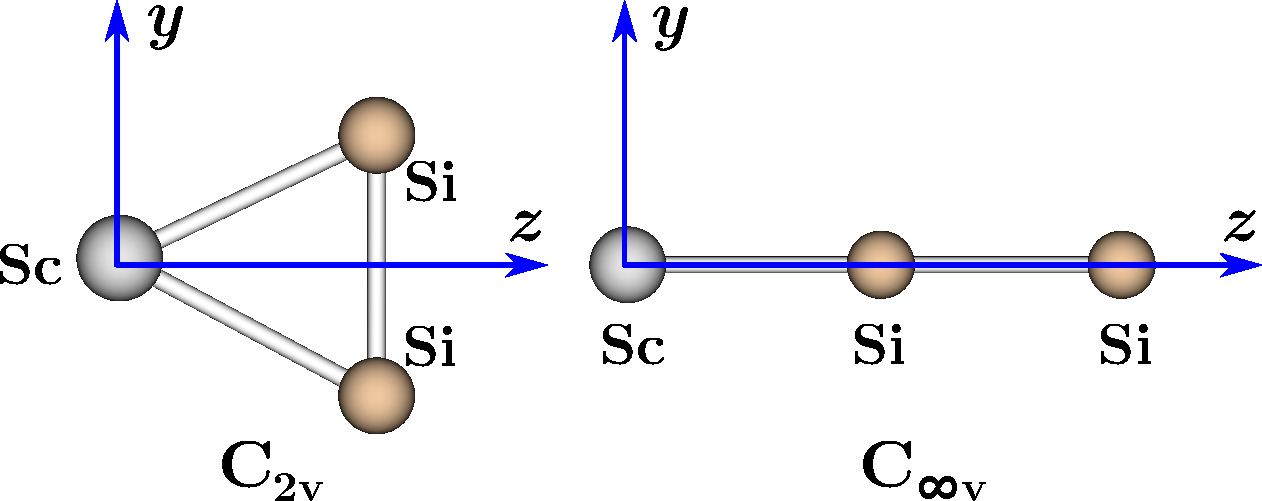
\includegraphics[width=0.5\textwidth]{scsi2}
	\caption{Two isomers of \ch{ScSi2^{-/0}} clusters and the coordinate systems used.}
	\label{fig3:scsi2}
\end{figure}





In the second step, the ground states of both anionic and neutral clusters \ch{ScSi2^{-/0}} are determined using several methods. Because the global ground states are crucial in solving the anion \acrshort{pe} spectrum, the identity and location of such states should correctly be determined on the potential energy surfaces. All states with regard to a spatial symmetry of the most stable structure, which was previously found, are optimized at higher levels of correlation energy. Owing to the employment of spatial symmetry, one needs to define a specific precoordinate system. Conventionally, the cyclic structure of \ch{ScSi2^{-/0}}, eventually proved to have C$_{2v}$ point group, and to be the most stable one, is graphically defined in Figure \ref{fig3:scsi2}, in which the Sc center is set to be the Cartesian coordinate origin and the yz-plane contains the cluster frame. Some additional \acrshort{caspt2} calculations for the linear isomer (Figure \ref{fig3:scsi2}) with symmetry of C$_\infty$$_v$ are calculated within the spatial symmetry of C$_{2v}$ because the nonabelian group C$_\infty$$_v$ is not supported in the quantum chemical packages used in this work.




In this work, we use the complete active space self-consistent field (\acrshort{casscf}) method to construct the wave functions that recover the nondynamic correlation well, and subsequently the second-order perturbation (\acrshort{caspt2}) method, based on \acrshort{casscf} wave functions as references, that takes into account the dynamical correlation parts. Hence, geometry optimizations of different electronic states are carried out using the \acrshort{casscf}/\acrshort{caspt2}.\cite{c3:40} This is in part because a few singlet open-shell states cannot be accessed by single reference methods, and consequently, cannot be geometrically optimized. From our preliminary evaluations, because the 3s and inner-shell orbitals of Si atoms are found not to be involved in the ionization processes causing experimental \acrshort{pe} bands, and more importantly to reduce computational costs of \acrshort{caspt2} optimizations, the 3s and all inner-shell orbitals of Si are not treated in the active space. Instead, six valence 3p orbitals of two Si atoms, together with six valence orbitals (five 3d and one 4s) of the scandium atom are included in the active space of \acrshort{casscf} calculations. Depending on the charge states of \ch{ScSi2}, the number of electrons included in the active space amounts to 7 and 8 for the neutral and anion, respectively. As a result, there are 12 orbitals in the active space for variable occupancy by 7 or 8 electrons. The number of configuration state functions produced in our \acrshort{casscf} calculations can be over 28.000 (for singlet states).




For calibration, single-point electronic energies at restricted single and double coupled cluster theory plus the perturbative contributions of connected triple excitations \acrshort{rccsd}(T) are also calculated at \acrshort{caspt2} geometries. A few additional multiconfigurational reference computations using internally contracted configuration interaction (\acrshort{mrci}(Q)) on the basis of \acrshort{casscf} wave functions making use of \acrshort{caspt2} geometries are also conducted to check further the conclusion on the global ground states. To obtain more reliable \acrshort{mrci}(Q) energies, each \acrshort{mrci} calculation takes into account all configuration state functions with coefficients larger than or equal to 0.01, and then the \acrshort{mrci} energies are corrected using the Davidson correction for the quadrupole contributions to correlation energies. At this step, the correlation consistent triple-$\zeta$ basis set aug-cc-PVTZ-DK is used for all single reference and \acrshort{mrci} calculations; the atomic natural orbital basis set \acrshort{ano}-RCC contracted to [7s6p4d3f2g]\cite{c3:41} for Sc and to [5s4p3d2f]\cite{c3:42} for Si is used in the \acrshort{casscf} and \acrshort{caspt2} calculations. In the evaluation of \acrshort{ade}s and \acrshort{vde}s, single-point B3LYP, BP86 and \acrshort{rccsd}(T) energies are equally obtained using a larger quintuple-$\zeta$ aug-cc-PV5Z-DK basis set,\cite{c3:37, c3:38} in which DK stands for the relativistic account. It should be noted that the \acrshort{ade}s are calculated at \acrshort{caspt2} optimized geometries of the corresponding states, whereas all the \acrshort{vde}s are evaluated at the \acrshort{caspt2} optimal geometry of the anionic ground state. For \acrshort{rccsd}(T), \acrshort{mrci}, and \acrshort{caspt2} computations, the inner-shell orbitals 1s, 2s, and 2p of Sc and 1s of Si atoms are not correlated. Scalar relativistic effects are treated by the mean of the second-order Douglas–Kroll–Hess Hamiltonian.\cite{c3:43} Single-point and optimization \acrshort{caspt2} calculations are performed using the MOLCAS 8.1 package,\cite{c3:44} and \acrshort{dft} , \acrshort{rccsd}(T), and \acrshort{mrci} are carried out with the aid of the MOLPRO 2012 package.\cite{c3:45} The true energy minima obtained from optimizations are confirmed by all positive harmonic vibrational frequencies. 




The last step of the present study is to simulate the band progressions in the anion photoelectron spectrum of \ch{ScSi2-}. Harmonic vibrational frequencies of four accessible neutral states corresponding to the X, A, B, and D bands are calculated at the B3LYP level as mentioned above. Such calculations also provide the equilibrium geometries and normal modes of vibration. By carrying out all possible integrations of the multidimensional Franck-Condon factors up to 15 quanta of many modes, we can theoretically evaluate relative intensities of peaks within each progression, as well as the width of such progressions. This result reveals a more detailed visualization of the bands in the spectrum. The calculations of integrals are implemented with the MolFC program.\cite{c3:46}



\section{Results and Discussion}


\subsection{Ground States and Low-Lying States of \ch{ScSi2^{-/0}}}

To ensure that the cyclic isomer with C$_{2v}$ point group corresponds to the most stable structures of both the anionic and neutral clusters as reported elsewhere,\cite{c3:9, c3:14, c3:16} optimization energies of many different spin-multiplicity states at the B3LYP and BP86 are calculated and visualized in Figure \href{https://pubs.acs.org/doi/suppl/10.1021/acs.jpca.6b09067/suppl_file/jp6b09067_si_001.pdf}{\textcolor{blue}{S1}} of the \href{https://pubs.acs.org/doi/suppl/10.1021/acs.jpca.6b09067/suppl_file/jp6b09067_si_001.pdf}{\textcolor{blue}{Supporting Information}} (available online). Apparently, the cyclic C$_{2v}$ isomer is found to be in each state more stable than the linear isomer. To be more detailed, a triplet and a doublet state are found to be the ground states of the anionic and the neutral clusters, respectively. It should be mentioned here that all high-spin states of the cyclic isomers (sextet, septet, and octet states), which are energetically much higher than the low-spin states of the anion and the neutral, are no longer considered in the next step. 




From previous calculations, the cyclic C$_{2v}$ form of the anion and the neutral have been determined as the most stable isomer, and therefore this geometrical structure is believed to be involved in experimental photodetachments. However, the ground state of the anionic cluster from which one electron is removed needs to be exactly known. For this reason, four triplet states ($^3$A$_1$, $^3$B$_1$, $^3$B$_2$ and $^3$A$_2$) of the cyclic isomer are taken into account in the geometrical optimizations. Four doublet states of the neutral cluster are also geometrically optimized for the search of the ground state. Geometrical optimizations of other energetic neighbors on the potential surfaces of the anion and the neutral are performed as well. The relative energies at the B3LYP, BP86, \acrshort{rccsd}(T), and \acrshort{caspt2} levels, and the \acrshort{caspt2} geometries used to compute \acrshort{rccsd}(T) energies are presented in Table \ref{tbl2:RE}. To be safer, we also calculated the relative energies of all singlet and triplet states of the linear isomer at the \acrshort{caspt2} level by doing geometrical optimizations and provide them in Table \href{https://pubs.acs.org/doi/suppl/10.1021/acs.jpca.6b09067/suppl_file/jp6b09067_si_001.pdf}{\textcolor{blue}{S1}} of the \href{https://pubs.acs.org/doi/suppl/10.1021/acs.jpca.6b09067/suppl_file/jp6b09067_si_001.pdf}{\textcolor{blue}{ESI} file}.




\begin{table}[htb!]
	\centering
	\begin{threeparttable} 
	\caption{Relative Energies and Structural Parameters of the Ground and Low-Lying States\tnote{(a)}}
	\label{tbl2:RE}
	\begin{tabular}{@{}lllcclcccc@{}}
	\toprule
	cluster  & state &  & \multicolumn{2}{c}{\acrshort{caspt2} geometry (\AA)} &  & \multicolumn{4}{c}{relative energy (eV)} \\ \cmidrule(r){1-2} \cmidrule(lr){4-5} \cmidrule(l){7-10} 
	 &        &  & Sc-Si & Si-Si &  & B3LYP   & BP86   & \acrshort{rccsd}(T)   & \acrshort{caspt2}   \\ \cmidrule(r){1-2} \cmidrule(lr){4-5} \cmidrule(l){7-10} 
	\multirow{12}{*}{\begin{tabular}[c]{@{}l@{}}cyclic\\ \\ \ch{ScSi2-}\end{tabular}} & $^1$A$_1$   &  & 2.666              & 2.142              &  & 0.54    & 0.64   & 0.03       & 0.28     \\
	 & $^1$B$_1$   &  & 2.404              & 2.356              &  &         &        &            & 0.81     \\
	 & $^1$B$_2$   &  & 2.500              & 2.237              &  &         &        &            & 0.07     \\
	 & $^1$A$_2$   &  & 2.694              & 2.143              &  &         &        &            & 0.37     \\
	 & $^3$A$_1$   &  & 2.725              & 2.138              &  & 0.45    & 0.68   & 0.34       & 0.30     \\
	 & $^3$B$_1$   &  & 2.408              & 2.439              &  & 0.59    & 0.48   & 0.72       & 0.50     \\
	 & $^3$B$_2$   &  & 2.479              & 2.250              &  & 0.00    & 0.00   & 0.00       & 0.00     \\
	 & $^3$A$_2$   &  & 2.701              & 2.140              &  & 0.31    & 0.43   & 0.24       & 0.24     \\
	 & $^5$A$_1$   &  & 2.601              & 2.345              &  & 1.28    & 1.21   & 1.37       & 1.49     \\
	 & $^5$B$_1$   &  & 2.423              & 2.415              &  & 1.32    & 1.24   & 1.63       & 1.56     \\
	 & $^5$B$_2$   &  & 2.746              & 2.173              &  & 1.49    & 1.57   & 1.59       & 1.70     \\
	 & $^5$A$_2$   &  & 2.748              & 2.167              &  & 1.58    & 1.64   & 1.64       & 1.80     \\ \cmidrule(r){1-2} \cmidrule(lr){4-5} \cmidrule(l){7-10} 
	\multirow{8}{*}{\begin{tabular}[c]{@{}l@{}}cyclic\\ \\ \ch{ScSi2^0} \end{tabular}}  & $^2$A$_1$   &  & 2.560              & 2.160              &  & 1.61    & 1.81   & 1.60       & 1.57     \\
	 & $^2$B$_1$   &  & 2.600              & 2.160              &  & 2.10    & 2.46   & 2.13       & 1.98     \\
	 & $^2$B$_2$   &  & 2.435              & 2.286              &  & 1.34    & 1.50   & 1.41       & 1.09     \\
	 & $^2$A$_2$   &  & 2.540              & 2.168              &  & 1.65    & 1.89   & 1.73       & 1.63     \\
	 & $^4$A$_1$   &  & 2.480              & 2.538              &  & 2.50    & 2.63   & 2.77       & 2.50     \\
	 & $^4$B$_1$   &  & 2.366              & 2.453              &  & 2.53    & 2.66   & 2.94       & 2.57     \\
	 & $^4$B$_2$   &  & 2.608              & 2.159              &  & 2.29    & 2.50   & 2.46       & 2.33     \\
	 & $^4$A$_2$   &  & 2.599              & 2.490              &  & 2.36    & 2.63   & 2.77       & 2.63     \\ \bottomrule
	\end{tabular}
	\begin{tablenotes}
		\item[(a)] Single-point \acrshort{rccsd}(T) energies were calculated using \acrshort{caspt2} optimized geometries. At the B3LYP, BP86, and \acrshort{caspt2} levels, energies are obtained with optimized geometries at the same level. These values are electronic energies without \acrshort{zpe}s. The basis sets aug-cc-PVTZ-DK (for single reference methods \acrshort{dft}  and \acrshort{rccsd}(T)) and \acrshort{ano}-RCC (for \acrshort{casscf}/\acrshort{caspt2}) were used including the scalar relativistic effects.
	\end{tablenotes}
	\end{threeparttable}
	\end{table}






Relative energies listed in Table \ref{tbl2:RE} indicate that the triplet $^3$B$_2$ has the lowest energy of the anion \ch{ScSi2-}. Indeed, all the remaining low-lying singlet and triplet states, as well as the higher spin states are higher in energy than that of the $^3$B$_2$ state at all levels considered. The \acrshort{caspt2} and \acrshort{rccsd}(T) adiabatically place the $^3$A$_2$ at 0.24 eV above the $^3$B$_2$, whereas the $^3$A$_1$ is positioned at $\sim$0.1 eV higher than $^3$A$_2$ at the \acrshort{rccsd}(T) level. When the four singlet states are considered, \acrshort{caspt2} calculations reveal that the open-shell $^1$B$_2$ state is just 0.07 eV above the $^3$B$_2$; such a small difference in energy is within the error margin of the \acrshort{caspt2} method. Additionally, the \acrshort{rccsd}(T) energy of the $^1$A$_1$ is only 0.03 eV above that of the $^3$B$_2$, although \acrshort{caspt2} energy of this state is 0.28 eV higher than that of the $^3$B$_2$ state. Such small differences in relative energies motivate us to perform additional multireference configuration interaction (\acrshort{mrci}) calculations for the states $^1$A$_1$,  $^1$B$_2$, and $^3$B$_2$. The internally contracted \acrshort{mrci} calculations, for a specific state, include more than one billion uncontracted configurations (being over 87 million contracted configurations) and are therefore very computationally expensive. Hence, \acrshort{mrci} calculations are only carried out for the necessary states mentioned above. \acrshort{mrci} calculations for the anion indicate that the $^3$B$_2$ state is 0.17 and 0.09 eV lower in energy than the $^1$A$_1$ and $^1$B$_2$ states, respectively. Overall, all results from \acrshort{dft} , \acrshort{rccsd}(T), \acrshort{caspt2}, and \acrshort{mrci} calculations allow us to conclude that the triplet $^3$B$_2$ is the ground state of the anionic cluster \ch{ScSi2-}, which confirms the result of a previous report.\cite{c3:16} This state exhibits the following orbital configuration: $^3$B$_2$ \ldots (12a$_1$)$^2$ (4b$_1$)$^2$ (13a$_1$)$^1$ (8b$_2$)$^1$. As for the neutral cluster, determination of its ground state appears to be more straightforward because all the doublet and quartet states are accessible from all quantum chemical methods. The \acrshort{dft}  (using B3LYP, BP86 functionals) and coupled-cluster theory \acrshort{rccsd}(T) methods identify the low-spin $^2$B$_2$ at $\sim$0.20 eV lower in energy than the $^2$A$_1$ state. \acrshort{caspt2} optimizations also determine the energy of $^2$B$_2$ to be lower than that of $^2$A$_1$, but the \acrshort{caspt2} relative energy gap is slightly larger with a difference of $\sim$0.5 eV between the $^2$B$_2$ and $^2$A$_1$. All high-spin quartet states of the cyclic neutral \ch{ScSi2} are about 1.20 eV energetically higher than $^2$B$_2$ at the \acrshort{dft} , \acrshort{rccsd}(T) and \acrshort{caspt2} levels. Unambiguously, the $^2$B$_2$ can be assigned as the ground state of the neutral cluster \ch{ScSi2}.\cite{c3:16}




\subsection{Electronic Structures and Possible One-Electron Detachments}




Because the electronic configurations of states decide the ionization processes, all of them are now thoroughly analyzed. By extracting leading configurations from the \acrshort{casscf} levels, we reveal the detailed electronic structures of possible initial and final states involving the ionization processes. In going from the ground states of both the anionic and neutral clusters \ch{ScSi2^{-/0}}, all other low-lying states that follow one-electron detachments, are investigated. All the leading configurations of selected states are tabulated in Table \ref{tbl3:leading}.


\begin{table}[]
	\small
	%\setlength\LTcapwidth{\textwidth} % default: 4in (rather less than \textwidth...)
	%\setlength\LTleft{0pt}            % default: \parindent
	%\setlength\LTright{0pt}           % default: \fill
	\centering
	\caption{\acrshort{casscf} Leading Configurations and Possible Ionization Processes Starting from the Anionic Ground State $^3$B$_2$, and from the Nearly Degenerate State $^1$B$_2$.}
	\label{tbl3:leading}
	\begin{threeparttable}
	%\begin{tabular}{@{\extracolsep{\fill}}lccll@{}}
	\begin{tabular}{@{}llcll@{}}
		\toprule
		state & leading configuration                   		        & weight (\%) & ionization  & ionization orbital  \\ \midrule
$^3$B$_2$ & 11a$_1^2$ 12a$_1^2$ 13a$_1^1$ 4b$_1^2$ 5b$_1^0$ 8b$_2^1$ 2a$_2^0$  & 87   &                                       &                      \\
$^1$B$_2$ & 11a$_1^2$ 12a$_1^2$ 13a$_1^1$ 4b$_1^2$ 5b$_1^0$ 8b$_2^1$ 2a$_2^0$  & 87   &                                       &                      \\
\multirow{2}{*}{$^2$A$_1$} & \multirow{2}{*}{11a$_1^2$ 12a$_1^2$ 13a$_1^1$ 4b$_1^2$ 5b$_1^0$ 8b$_2^0$ 2a$_2^0$} & \multirow{2}{*}{85} & $^3$B$_2$ $\longrightarrow$ $^2$A$_1$    & \multirow{2}{*}{8b$_2$ (Sc: 3d$_{yz}$)} \\
		      &                                         &                             & $^1$B$_2 \longrightarrow ^2$A$_1$\tnote{(b)} &              \\
$^2$B$_1$  & 11a$_1^2$ 12a$_1^2$ 13a$_1^0$ 4b$_1^2$ 5b$_1^1$ 8b$_2^0$ 2a$_2^0$  & 88  &                                      &                      \\
$^2$B$_2$  & 11a$_1^2$ 12a$_1^2$ 13a$_1^0$ 4b$_1^2$ 5b$_1^0$ 8b$_2^1$ 2a$_2^0$  & 85  & $^3$B$_2 \longrightarrow ^2$B$_2$    & 13a$_1$ (Sc: 4s)     \\
$^2$A$_2$  & 11a$_1^2$ 12a$_1^2$ 13a$_1^0$ 4b$_1^2$ 5b$_1^0$ 8b$_2^0$ 2a$_2^1$  & 87  &                                      &                      \\
1$^4$A$_1$ & 11a$_1^2$ 12a$_1^2$ 13a$_1^0$ 4b$_1^1$ 5b$_1^0$ 8b$_2^1$ 2a$_2^1$  & 83  &                                      &                      \\
1$^4$B$_1$ & 11a$_1^1$ 12a$_1^2$ 13a$_1^0$ 4b$_1^2$ 5b$_1^0$ 8b$_2^1$ 2a$_2^1$  & 87  &                                      &                      \\
1$^4$B$_2$ & 11a$_1^2$ 12a$_1^1$ 13a$_1^1$ 4b$_1^2$ 5b$_1^0$ 8b$_2^1$ 2a$_2^0$  & 89  & $^3$B$_2 \longrightarrow$ 1$^4$B$_2$ & 12a$_1$ (Si: 3p$_y$) \\
2$^4$B$_2$ & 11a$_1^1$ 12a$_1^2$ 13a$_1^1$ 4b$_1^2$ 5b$_1^0$ 8b$_2^1$ 2a$_2^0$  & 84  & $^3$B$_2 \longrightarrow$ 2$^4$B$_2$ & 11a$_1$ (Si: 3p$_z$) \\
1$^4$A$_2$ & 11a$_1^2$ 12a$_1^2$ 13a$_1^1$ 4b$_1^1$ 5b$_1^0$ 8b$_2^1$ 2a$_2^0$  & 86  & $^3$B$_2 \longrightarrow    ^4$A$_2$ & 4b$_1$  (Si: 3p$_x$) \\ \bottomrule
	\end{tabular}
	\begin{tablenotes}
		\item[(b)] This transition is considered when the nearly degenerate state $^1$B$_2$ is supposed to be populated.
	\end{tablenotes}
	\end{threeparttable}
\end{table}





The $^3$B$_2$ ground state has three doubly and two singly occupied orbitals in the active space. Whereas two singly occupied orbitals 13a$_1$ and 8b$_2$ are mostly contributed from Sc valence orbitals 4s and 3d$_{yz}$, three doubly occupied ones originate from $\pi_u$ (11a$_1$ and 4b$_1$) and $\sigma_g$ (12a$_1$) orbitals of the \ch{Si2-} ligand. These ligand orbitals dominantly constitute the 3p orbitals from Si atoms, which are 3p$_x$ and 3p$_z$ for the case of two $\pi_u$ orbitals, and are 3p$_y$ for the case of $\sigma_g$. 




The leading configuration of $^3$B$_2$ can also be written as [\ldots $\pi^2_{3p_z}$ $\sigma^2_{3p_y}$ 4$s^1$ $\pi^2_{3p_x}$ 3$d^1_{yz}$] in terms of dominant orbital contributions. Similarly, the $^2$B$_2$ state can be analyzed from its obtained leading configuration. Most features of active orbitals are the same as those of the $^3$B$_2$. Nevertheless, instead of two metallic singly occupied orbitals as the case of $^3$B$_2$, the $^2$B$_2$ state has only one singly occupied one (8b$_2$). This is originally the 3d$_{yz}$ orbital of Sc. It means that an electron in the 4s orbital is removed from the $^3$B$_2$ state to form the $^2$B$_2$ if the ionization process happens during the measurement of anion photoelectron spectra. This one-electron removal can obviously be seen by comparing the leading configurations between these states. As a result, the leading configuration of $^2$B$_2$ can be described as [\ldots $\pi^2_{3p_z}$ $\sigma^2_{3p_y}$ 4$s^0$ $\pi^2_{3p_x}$ 3$d^1_{yz}$]. For an intuitive visualization, the pseudonatural active orbitals of these two states are plotted in Figure \ref{fig3:orbs}. The ionization process is thus denoted as $^3$B$_2$ $\longrightarrow$ $^2$B$_2$ together with the corresponding ionization orbital 13a$_1$ (Sc: 4s) in Table \ref{tbl3:leading}.


\begin{figure}[htb!]
	\centering
	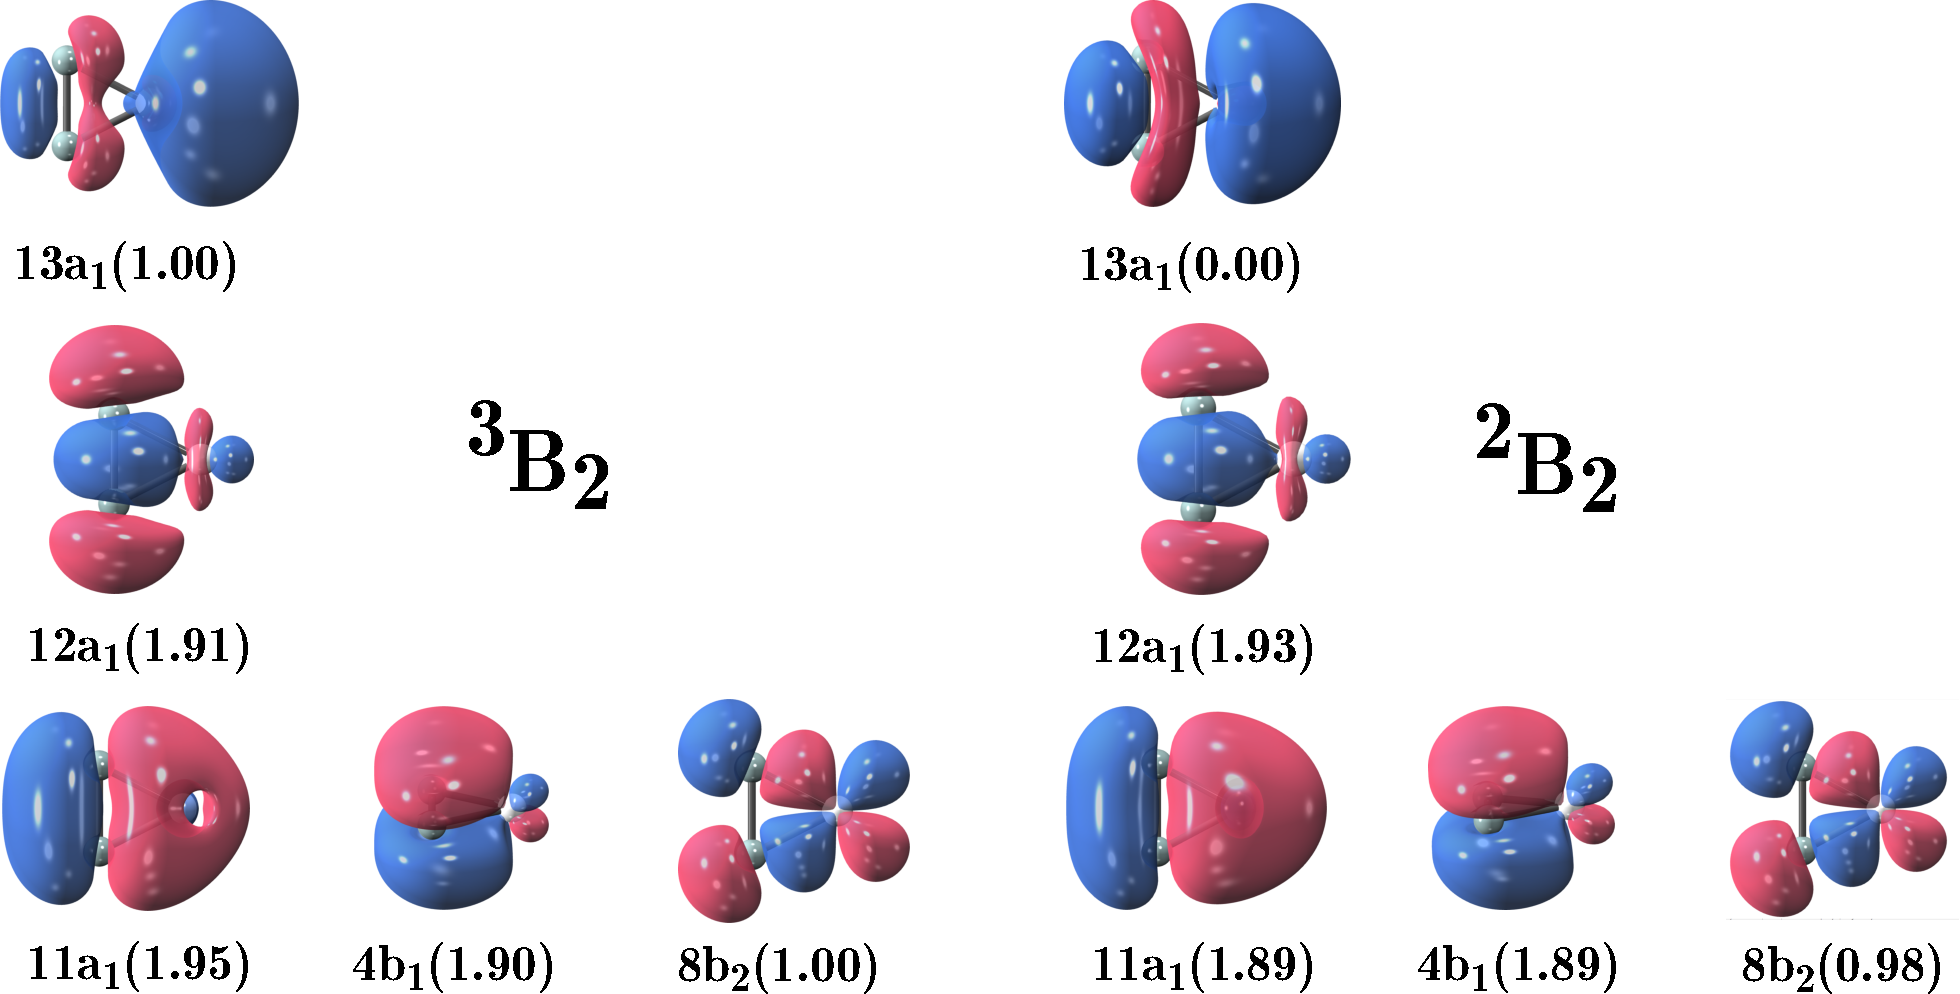
\includegraphics[width=0.8\textwidth]{3B2-2B2-orbitals}
	\caption{Occupied \acrshort{casscf} pseudonatural active orbitals of $^3$B$_2$ and corresponding active orbitals of $^2$B$_2$. Average occupation numbers are given in parentheses. Scandium atoms are on the right-hand side of each cluster.}
	\label{fig3:orbs}
\end{figure}



As mentioned above, with regard to the one-electron detachment process, if the $^3$B$_2$ state is the ground state of the anionic cluster, the final state can be a state of doublet and of quartet. Thus, besides the neutral ground state $^2$B$_2$, other doublet states and the quartet states should be examined. By considering the leading configurations, we can predict the $^2$A$_1$ state as a final state of the ionization process starting from the $^3$B$_2$. In fact, two leading configurations of $^3$B$_2$ and $^2$A$_1$ are just distinguishable from each other through the $^8$b$_2$ orbital, which is singly occupied in the state of $^3$B$_2$ and unoccupied in the latter state. Therefore, this one-electron detachment should appear somewhere in the anion photoelectron spectrum of \ch{ScSi2-}. For two other leading configurations $^2$B$_1$ and $^2$A$_2$, both cannot be the final states, because these leading configurations are not the consequences of one-electron detachments starting from the anionic ground state $^3$B$_2$. Up to now, two ionization processes can happen upon excitation of the 4s and 3d$_{yz}$ electrons, which are valence orbitals of Sc.  



Concerning the quartet states, three singly occupied orbitals with particular symmetrical orbitals decide the electronic state of the neutral cluster. When comparing the leading configurations of both 1$^4$A$_1$ and 1$^4$B$_1$ with the anionic ground state $^3$B$_2$, one can point out that no one-electron detachments from $^3$B$_2$ are possible to produce these two leading configurations. This can be understood by electron occupation in the orbital 2a$_2$, which has a large contribution from the 3d$_{xy}$(Sc) orbital. Indeed, though the orbital 2a$_2$ is unoccupied in the $^3$B$_2$ state, it is singly occupied in both 1$^4$A$_1$ and 1$^4$B$_1$ states. There are also differences in occupancy of orbitals in the representations a$_1$ and b$_1$ between the $^3$B$_2$ and these two quartet states. Let us recall that two metallic orbitals 13a$_1$ and $^8$b$_2$ are found to be the key orbitals involving in the above-mentioned ionization processes. Therefore, removals of electrons from the 3p(Si) orbitals are expected to appear in the photoelectron spectrum of \ch{ScSi2-} as well. 



With the electronic structure of the $^3$B$_2$ state, the tentative final states corresponding to three one-electron removals from three bonding orbitals $\pi_{3p_x}$, $\pi_{3p_z}$, $\sigma_{3p_y}$ can be predicted. Clearly, if the ionization happens upon removal of one electron from the bonding orbital $\sigma_{3p_y}$ (12a$_1$) in the ligand, the obtained leading configuration is that of 1$^4$B$_2$. Similarly, if one-electron transition starts from the bonding orbital $\pi_{3p_z}$ (11a$_1$), the electronic structure of 2$^4$B$_2$ is observed. For the 1$^4$A$_1$ state, the one-electron transition is out of the totally symmetrical a$_1$ orbitals but not the b$_1$ one. Instead of a doubly occupied orbital, the 4b$_1$ orbital, dominantly composed of the $\pi_{3p_x}$ orbital of the \ch{Si2} moiety, is a singly occupied one. This suggests that removal of one electron can occur at the 4b$_1$ orbital, and this should be reflected in the photoelectron spectrum of \ch{ScSi2-}. All the one-electron transitions and ionization orbitals can be found in Table \ref{tbl3:leading}.



The charge distribution among the atoms in the anionic ground state $^3$B$_2$ can be drawn from its electronic structure. First, the electronic structure of \ch{Si2-} should be considered. The ground state of the diatomic anion \ch{Si2-} was, originally, reported to be 2$\pi_u$, whose configuration was written as [\ldots $\pi^3_u\sigma^2_g$].\cite{c3:47} Later, a revision suggested that the nearly degenerate state $^2\Sigma_g^+$ with configuration of [\ldots $\pi^4_u\sigma^1_g$] is the ground state.\cite{c3:48}  This result is in better agreement with a previous study.\cite{c3:49} Technically, these configurations can be interpreted as the states [\ldots ($\pi_{3p_x}\pi_{3p_z}$)$^3$ $\sigma^2_{3p_y}$] and [($\pi_{3p_x} \pi_{3p_z}$)$^4$ $\sigma^1_{3p_y}$] for $^2\pi_u$ and $^2\Sigma_g^+$, respectively, if the coordinate system of the C$_{2v}$ isomer presented in Figure \ref{fig3:scsi2} is applied to the \ch{Si2-} unit. In each of these two nearly degenerate configurations, there are in total five electrons occupying two degenerate $\pi_u$ orbitals and a $\sigma_g$ one. Because these two nearly degenerate states are believed to be experimentally populated,\cite{c3:48} they can be involved in the formation process of the anion \ch{ScSi2-}. As seen in the electronic configuration of the $^3$B$_2$ ground state [\ldots $\pi^2_{3p_z}$ $\sigma^2_{3p_y}$ 4$s^1$ $\pi^2_{3p_x}$ 3$d_{yz}^1$], all orbitals of the \ch{Si2-} ligand are doubly occupied. The electronic configurations of two nearly degenerate states of \ch{Si2-} and the ground state of \ch{ScSi2-} provide unequivocal evidence proving that one electron in the valence orbitals of Sc is attracted and captured by the \ch{Si2} moiety, even though the mechanism of electron transfer is different with regard to which state of \ch{Si2-} reacting with Sc atoms. This allows us to suggest the formal oxidation states of each components in the anionic cluster \ch{ScSi2-} as \ch{(Sc)^{+1}(Si_2)^{-2}}. With the same line of thought, the formal oxidation states of the Sc and  \ch{Si2} parts in two neutral states $^2$A$_1$ and $^2$B$_2$ can be described as \ch{(Sc)^{+2}(Si2)^{-2}}, because one electron is removed from the metallic orbitals of Sc during the ionization. It becomes different for three quartet states, 1$^4$B$_2$, 2$^4$B$_2$, and 1$^4$A$_2$. As the ionization processes start from $\sigma^2_{3p_y}$, $\pi^2_{3p_x}$ and $\pi^2_{3p_z}$ of the ligand, the formal oxidation states of \ch{Si2} moiety should be -1. As a result, the formal oxidation states of these three quartet states can be described as \ch{(Sc)^{+1}(Si2)^{-1}}. 




These charge distributions can also be easily obtained from population analyses. The Bader charges of Sc and Si atoms analyzed at the \acrshort{casscf} wave functions are provided in Table \ref{tbl3:charge}. The \acrshort{aim} charge values afford a better description of charge distribution among Sc and Si atoms. The most obvious feature is the actual values of charge correctly reflect the signs of formal oxidation states, which are positive for Sc and negative for Si. The absolute values of charge also well demonstrate the charge redistribution when one electron is removed from a specific moiety of the anionic ground state $^3$B$_2$. To be more detailed, the absolute charge value on the Sc atom is somewhat in balance with that on each Si atom (0.56 versus 0.78) as their formal oxidation states are. When one electron is removed from Sc to form the doublet states $^2$A$_1$ and $^2$B$_2$, the positive charge of Sc increases to around +1.0 electron. This is what can be expected after considering changes in the formal oxidation states given above. A point of interest here is that the negative charge on Si tends to decrease. This can be understood by relaxation happening immediately after ionization. For a charge redistribution after detachments of an electron from \ch{Si2} moiety, the absolute value of negative charge on Si atoms is significantly reduced to approximate 0.4 electron as observed in two quartet states 1$^4$B$_2$ and 1$^4$A$_2$.




\begin{table}[htbp!]
	\centering
	\caption{Atomic Net Charges of Sc and Si (\acrshort{casscf})}
	\label{tbl3:charge}
	\begin{tabular}{@{}lccc@{}}
	\toprule
	\multirow{2}{*}{state} 		 & \multicolumn{3}{c}{\acrshort{aim} charge (electron)} \\ \cmidrule(l){2-4} 
						   		 & Sc           & Si           & Si          \\ \midrule
	$^3$B$_2$                    & +0.56        & -0.78        & -0.78       \\
	$^2$A$_1$                    & +0.96        & -0.48        & -0.48       \\
	$^2$B$_2$                    & +1.06        & -0.53        & -0.53       \\
	1$^4$B$_2$                   & +0.82        & -0.41        & -0.41       \\
	1$^4$A$_2$                   & +0.84        & -0.42        & -0.42       \\ \bottomrule
	\end{tabular}
\end{table}



\subsection{Anion photoelectron Spectrum and Band Assignments}


With all possible one-electron ejections analyzed above, one can now evaluate the number of the first few anion photoelectron bands that can appear in the experimental spectrum of \ch{ScSi2-}. However, this type of qualitative information cannot be used to locate the energetic range of each one-electron detachment. In other words, the experimentally recorded bands cannot be assigned without extra ionization energies of these one-electron transitions. Thus, the \acrshort{ade}s and \acrshort{vde}s are of utmost importance in band assignments. Before considering this, for the sake of convenience, five experimental bands in the spectrum of \ch{ScSi2-}, reproduced in Figure \ref{fig3:spectrum}, can be labeled as X -- D. All calculated \acrshort{ade}s and \acrshort{vde}s at the \acrshort{dft} , \acrshort{rccsd}(T) and \acrshort{caspt2} levels of theory are presented in Table \ref{tbl3:DE}.


\begin{figure}[htb!]
	\centering
	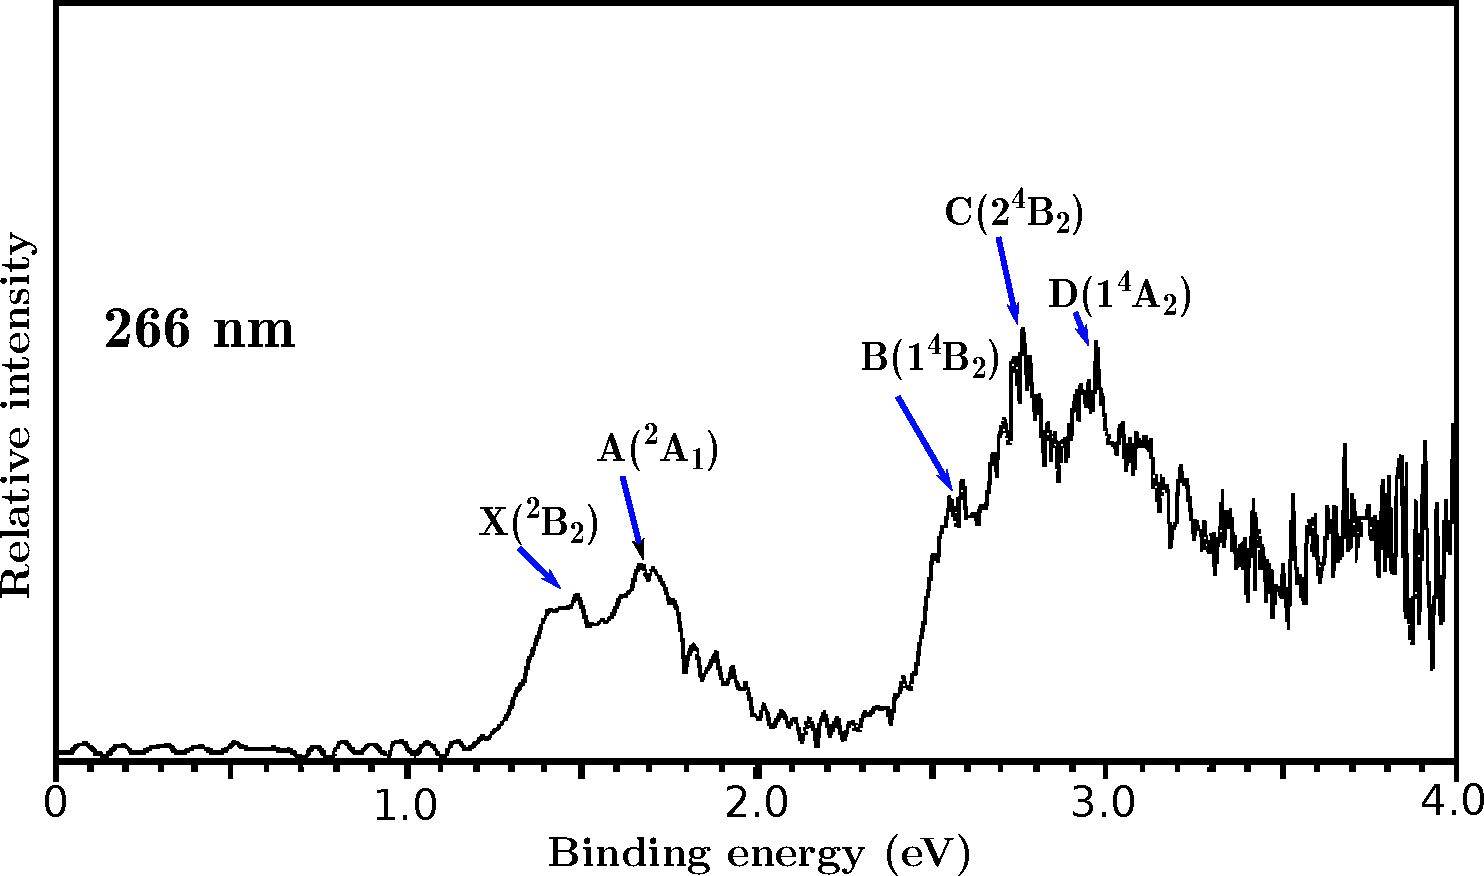
\includegraphics[width=0.8\textwidth]{spectrum}
	\caption{Anion photoelectron spectrum of \ch{ScSi2-} recorded at the photon energy of 266 nm (reproduced with permission from ref \citenum{c3:14}. Copyright 2011, CPS). Five bands in the spectrum are labeled as the traditional nomenclature of anion photoelectron bands (X -- D).}
	\label{fig3:spectrum}
\end{figure}



Normally, the lowest band X in an anion \acrshort{pe} spectrum is expected to be the result of a one-electron transition between the anionic and neutral ground states. For \ch{ScSi2-}, the transition $^3$B$_2$ $\longrightarrow$ $^2$B$_2$ is responsible for such a band. The calculated \acrshort{ade} and \acrshort{vde} at \acrshort{dft} , \acrshort{rccsd}(T), and \acrshort{caspt2} levels are in fact in good agreement with experimental values. All single reference methods predict the \acrshort{ade} and \acrshort{vde} deviations of about 0.10 eV from the experimental ones. Indeed, the experimental \acrshort{ade} of the X band is 1.28 eV, and the B3LYP, BP86, and \acrshort{rccsd}(T) \acrshort{ade}s are, respectively, estimated to be 1.31, 1.47, and 1.40 eV. The B3LYP and \acrshort{rccsd}(T) estimated values are much closer to the experimental \acrshort{ade} of 1.47 eV reported elsewhere. \cite{c3:16} The \acrshort{vde}s calculated again confirm the assignment for the X band when they are quite close to the experimental \acrshort{vde} of 1.44 eV. It is worth mentioning here that the \acrshort{caspt2} energy predictions of the \acrshort{ade} and \acrshort{vde} are slightly underestimated in comparison to the experimental ionization values (1.09 versus 1.28 eV for the \acrshort{ade}, and 1.17 versus 1.44 eV for the \acrshort{vde}). However, the differences in \acrshort{ade} and \acrshort{vde} between the \acrshort{caspt2} and experimental values (0.19 and 0.27 eV) are all below the error margin of the \acrshort{caspt2} method. All estimated \acrshort{vde}s and \acrshort{ade}s from single-reference methods for this band are in good agreement with experiment. This can be, in part, explained by the strong single-reference feature of the anionic and neutral ground states, which are quantitatively determined by the leading configurations weights listed in Table \ref{tbl3:leading}. For the other low-lying doublet states, the \acrshort{vde}s and \acrshort{ade}s are significantly higher than the experimental values. Therefore, $^2$B$_2$ is the unique state leading to the X band.






\begin{landscape}
	\begin{table}[htb!]
	\centering
	%\tiny
	\setlength\LTcapwidth{\textwidth} % default: 4in (rather less than \textwidth...)
	\setlength\LTleft{0pt}            % default: \parindent
	\setlength\LTright{0pt}           % default: \fill
	\begin{threeparttable}
	\caption{Adiabatic Detachment Energies and Vertical Detachment Energies Calculated at \acrshort{caspt2} Geometries in Table \ref{tbl3:leading}\tnote{(c)}}
	\label{tbl3:DE}                                                                
	\begin{tabular}{@{\extracolsep{\fill}}lccccccccccc@{}}
	\toprule
	\multirow{2}{*}{state} & \multicolumn{5}{c}{\acrshort{ade} (eV)}&  	   & \multicolumn{5}{c}{\acrshort{vde} (eV)}            \\ \cmidrule(lr){2-6} \cmidrule(l){8-12} 
				  & B3LYP & BP86 & \acrshort{rccsd}(T) & \acrshort{caspt2}      & exptl  &  & B3LYP & BP86 & \acrshort{rccsd}(T) & \acrshort{caspt2}      & exptl    \\ \cmidrule(r){1-6} \cmidrule(l){8-12} 
	$^3$B$_2$     & 0.00  & 0.00 & 0.00     & 0.00        &        &  & 0.00  & 0.00 & 0.00     & 0.00        &          \\
	$^1$B$_2$     &       &      &          & 0.07        &        &  &       &      &          & 0.08        &          \\
	$^2$A$_1$     & 1.54  & 1.76 & 1.63     & 1.57 (1.51) &        &  & 1.68  & 1.88 & 1.75     & 1.65 (1.55) & 1.69 (A) \\
	$^2$B$_1$     & 2.02  & 2.40 & 2.08     & 1.98        &        &  & 2.24  & 2.56 & 2.28     & 2.14        &          \\
	$^2$B$_2$     & 1.31  & 1.47 & 1.40     & 1.09        & 1.28   &  & 1.26  & 1.44 & 1.36     & 1.17        & 1.44 (X) \\
	$^2$A$_2$     & 1.57  & 1.84 & 1.68     & 1.63        &        &  & 1.65  & 1.86 & 1.75     & 1.69        &          \\
	1$^4$A$_1$    & 2.50  & 2.62 & 2.82     & 2.50        &        &  & 2.56  & 2.74 & 2.90     & 2.67        &          \\
	1$^4$B$_1$    & 2.65  & 2.73 & 2.92     & 2.57        &        &  & 2.50  & 2.63 & 2.82     & 2.71        &          \\
	1$^4$B$_2$    & 2.22  & 2.45 & 2.50     & 2.33        &        &  & 2.42  & 2.62 & 2.67     & 2.57        & 2.57 (B) \\
	2$^4$B$_2$    &       &      &          &             &        &  &       &      & 2.77     & 2.70        & 2.75 (C) \\
	1$^4$A$_2$    & 2.45  & 2.71 & 2.83     & 2.63        &        &  & 2.51  & 2.78 & 2.89     & 2.91        & 2.79 (D) \\ \bottomrule
\end{tabular}
	\begin{tablenotes}
	\item[(c)] All single reference calculations use the quintuple-$\zeta$ basis set aug-cc-pV5Z-DK. \acrshort{caspt2} energies are calculated by employing the same \acrshort{ano}-RCC basis set used in determination of the ground states. The values in the parentheses are the \acrshort{ade} and \acrshort{vde} of the supposed electronic transition $^1$B$_2 \longrightarrow ^2$A$_1$.
	\end{tablenotes}
	\end{threeparttable}   
\end{table}                                                                    
\end{landscape}


Because there are no experimental \acrshort{ade}s of the four bands A, B, C, and D, their assignments can only be made on the basis of \acrshort{vde}s. As stated above, removal of one electron from the 4s(Sc) orbital of the anionic ground state $^3$B$_2$ was proved to cause the appearance of the X band. In a logical aspect, removal of an electron from the 3d(Sc) orbital is expected to be the insight of the A band, because this band has the second lowest ionization energy. This view is reinforced by the detachment energies calculated at \acrshort{dft} , \acrshort{rccsd}(T), and \acrshort{caspt2} levels. The experimental \acrshort{vde} of the A band is 1.69 eV, which is very close to the B3LYP, \acrshort{rccsd}(T), and \acrshort{caspt2} values of 1.68, 1.75, and 1.65 eV, respectively, for the transition $^3$B$_2$ $\longrightarrow$ $^2$A$_1$. The pure exchange-correlation functional BP86 is not as accurate as the other methods, but its evaluation is still valuable as the deviation is 0.19 eV. As a consequence, the A band is safely attributed to the transition $^3$B$_2$ $\longrightarrow$ $^2$A$_1$, which is totally allowed by the one-electron detachment rule mentioned above. It is noticeable to mention that the leading configuration’s weight of the state $^2$A$_1$ is 85$\%$, which is the same as that of the neutral ground state $^2$B$_2$. As a result, this neutral state can electronically and energetically be well described with a single electron configuration.



Three remaining bands in the experimental spectrum are expected to be the results of detachments starting from three occupied orbitals $\pi_{3p_z}$, $\pi_{3p_x}$ and $\sigma_{3p_y}$ that are mainly located in the ligand \ch{Si2-}. When only the energies of orbitals in the intact diatomic anion \ch{Si2-} are considered, two degenerate orbitals $\pi_{3p_z}$ and $\pi_{3p_x}$ are the \acrshort{homo}s; and the orbital $\sigma_{3p_y}$ is the \acrshort{homo}-1.\cite{c3:47, c3:48, c3:49} When \ch{Si2-} combines with a Sc atom to form \ch{ScSi2-}, these orbitals slightly change, in part due to the interference of the same symmetrical orbitals from the transition metal Sc. Particularly, the \acrshort{casscf} pseudonatural orbitals show that $\sigma_{3p_y}$ has tiny contribution from the 3d$_{z^2}$ orbital; the $\pi_{3p_z}$ is contaminated by the 4s orbital, and the 3d$_{xz}$ partially places itself into the $\pi_{3p_x}$. As a result, the $\pi_{3p_z}$ and $\pi_{3p_x}$ which are actually the orbitals 11a$_1$ and 4b$_1$ in the leading configuration of the state $^3$B$_2$, are no longer degenerate, as these two orbitals are contributed by two types of orbitals with different levels of energy (4s and 3d). Because the level of 4s energy is lower than that of the 3d in the first-row \acrshort{tm}s, the energy level of $\pi_{3p_z}$ (11a$_1$) should be predictably lower than that of the $\pi_{3p_x}$ (4b$_1$). Thus, removal of an electron from the orbital 11a$_1$ of the anionic ground state $^3$B$_2$ needs less energy than that from the 4b$_1$ orbital. These basic considerations yield a clearer route to reach the final assignments for three remaining bands B, C and D. 



First, we find out the insight of the B band. Our calculated results identify that the transition $^3$B$_2$ $\longrightarrow$ 1$^4$B$_2$, which corresponds to the removal of an electron from the orbital $\sigma_{3p_y}$ (12a$_1$), has the lowest \acrshort{vde}. The methods BP86, \acrshort{rccsd}(T), and \acrshort{caspt2} predict this \acrshort{vde} to be 2.62, 2.67, and 2.57 eV, whereas the experimental \acrshort{vde} is 2.57 eV. In this case, the B3LYP value of 2.42 eV is underestimated. For the C and D bands, we can undoubtedly assign them to the formation of the 2$^4$B$_2$ and 1$^4$A$_2$ states, respectively, by taking the above analysis into account. For the state 2$^4$B$_2$, the \acrshort{vde} of the transition $^3$B$_2 \longrightarrow 2^4$B$_2$ is well obtained at \acrshort{rccsd}(T) and \acrshort{caspt2} levels but not at \acrshort{dft}  levels. Specifically, the \acrshort{rccsd}(T) detachment energy gives the best value of 2.77 eV for this ionization, which is only 0.02 eV larger than the experimental value of 2.75 eV and is larger than the \acrshort{caspt2} ionization energy an amount of 0.07 eV. 




With regard to the last band D, both \acrshort{rccsd}(T) and \acrshort{caspt2} values of 2.89 and 2.91 eV again accurately reproduce the experimental \acrshort{vde}s of 2.79 eV for the transition $^3$B$_2$ $\longrightarrow$ 1$^4$A$_2$. The pure BP86 functional also can correctly predict the detachment energy of 2.78 eV for the excited state 1$^4$A$_2$ of the neutral cluster \ch{ScSi2}. The hybrid B3LYP functional seriously underestimates this \acrshort{vde} by up to 0.30 eV below the experimental counterpart, though it predicts better detachment energies for the lower excited states. In summary, all the anion \acrshort{pe} bands in the spectrum of \ch{ScSi2-} are now assigned, and these assignments are denoted in Figure \ref{fig3:spectrum}.




As mentioned above, the $^1$B$_2$ is a nearly degenerate state of the ground state $^3$B$_2$. Therefore, this state can be populated during the anion \acrshort{pe} measurement. From the leading configuration of $^1$B$_2$, which is quite similar to that of $^3$B$_2$ except for spin of the electron in the singly occupied orbital 8b$_2$, and from other neutral states given in Table \ref{tbl3:leading} we can infer that the tentative state $^2$A$_1$ can be obtained only by removing the 3d$_{yz}$ electron from the 8b$_2$ orbital of $^1$B$_2$. Our \acrshort{caspt2} calculation predicted the transition $^1$B$_2$ $\longrightarrow$ $^2$A$_1$ has a \acrshort{vde} of 1.55 eV, which is energetically located in the range between X and A bands in the spectrum of \ch{ScSi2-}. On the basis of Maxwell-Boltzmann statistics, the energy splitting of two anionic nearly degenerate states and the cooled condition of \ch{ScSi2-} clusters obtained from the experiment,\cite{c3:14} one can expect that  the population of $^1$B$_2$ (a few percent) is very small in comparison to the ground state $^3$B$_2$. Therefore, one-electron transitions, if experimentally observed, starting from $^1$B$_2$ are believed to be not intense compared to those starting from the ground state $^3$B$_2$. This allows us to expect the intensity of the transition $^1$B$_2$ $\longrightarrow$ $^2$A$_1$ is negligible and can be overshadowed by the allowed transitions underlying the X and A bands in the spectrum. 





It is clear that most single reference methods can closely reproduce the experimental ionization energies of \ch{ScSi2-}. In conjunction with the leading configurations weights, around 85$\%$ for all states as listed in Table \ref{tbl3:leading}, one can safely conclude that the electronic structure of \ch{ScSi2^{-/0}} are basically single configurations. And thus, single-reference methods such as \acrshort{dft} , which are computationally more economic, can be used to correctly describe the ground and low-lying electronic states of \ch{ScSi2^{-/0}} clusters, except for the singlet open-shell states which are inaccessible by single reference methods.




\subsection{Franck-Condon Factor Simulations}


In an attempt to provide a clearer view of the photoelectron spectrum, simulations of multidimensional Franck–Condon factors for the four observed bands, whose harmonic vibrations of normal modes of the final states are computationally accessible, are carried out. Table \ref{tbl3:freq} collects the vibrational frequencies of normal modes and equilibrium geometries of relevant states for the Franck–Condon factor integration. On the basis of multidimensional Franck–Condon factors, the progressions occurring along the appearance of the four specific electronic transitions underlying the X, A, B, and D bands are depicted (Figure \ref{fig3:FC}).



\begin{table}[htbp!]
	\centering
	\caption{Equilibrium geometries and harmonic vibrational frequencies (B3LYP/aug-cc-pVTZ-DK) for the initial anionic state $^3$B$_2$ and four neutral final states corresponding to the bands X, A, B and D in the \acrshort{pe} spectrum}
	\label{tbl3:freq}
	\begin{tabular}{@{}lcccc@{}}
	\toprule
	\multirow{2}{*}{state} & \multicolumn{2}{l}{B3LYP geometry (\AA)} & \multirow{2}{*}{B3LYP frequencies (cm$^{-1}$)} & \multirow{2}{*}{band} \\ \cmidrule(lr){2-3}
	& Sc-Si       & Si-Si    &         &                          \\ \midrule
	$^3$B$_2$     & 2.59     & 2.21    & 227, 289, 450     &       \\
	$^2$A$_1$     & 2.59     & 2.16    & 220, 327, 547     & A     \\
	$^2$B$_2$     & 2.50     & 2.23    & 233, 334, 489     & X     \\
	1$^4$B$^2$    & 2.67     & 2.17    & 246, 265, 517     & B     \\
	1$^4$A$^2$    & 2.68     & 2.30    & 218, 256, 444     & D     \\ \bottomrule
	\end{tabular}
\end{table}


\begin{figure}[htb!]
	\centering
	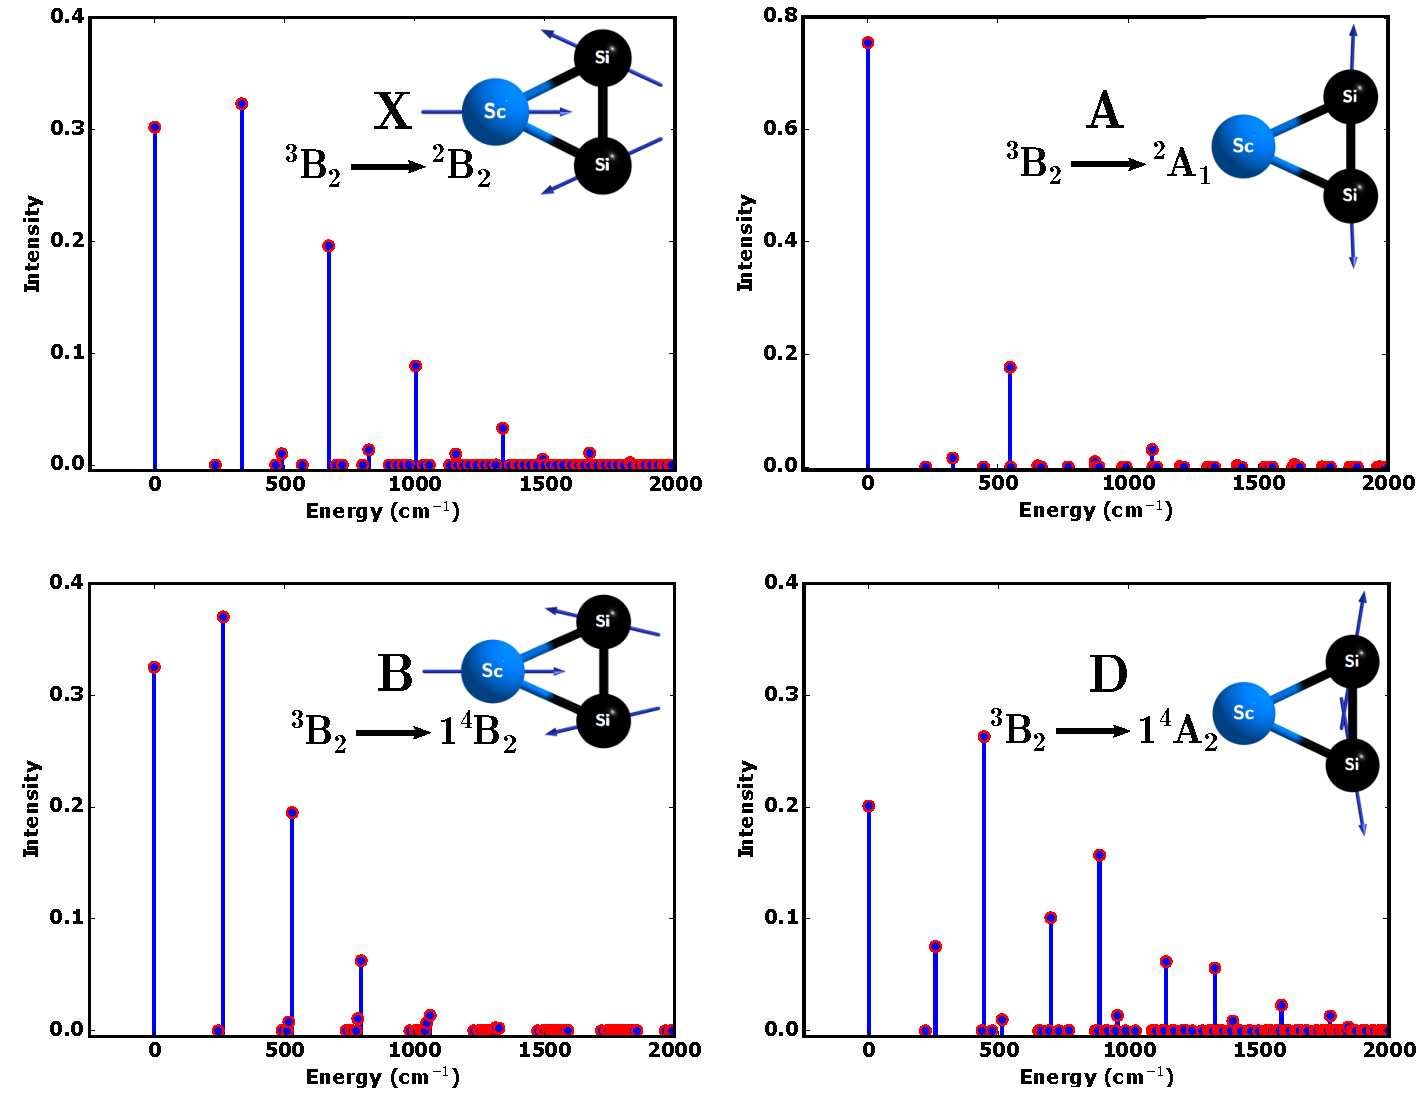
\includegraphics[width=\textwidth]{Franck-Condon}
	\caption{Franck-Condon factor simulations for the four bands X, A, B, and D of the photoelectron spectrum of \ch{ScSi2-}.}
	\label{fig3:FC}
\end{figure}





In the experimental bands, the exact number of peaks cannot be obtained and relative intensities of peaks within every band are not well-resolved. Thus, it is not possible to draw a detailed comparison between the experimental and the simulated bands. Theoretically, the X, B, and D band progressions are broader than band A, as visualized in Figure \ref{fig3:FC}. Such a difference in the progression broadening is due to the geometrical differences between the anionic ground state $^3$B$_2$ and the corresponding final neutral states. Particularly, at the vibrational frequency of 334 cm$^{-1}$, the reduction of the \ch{Sc-Si} bond from 2.59 to 2.50 \AA{} seems to be a key factor deciding the wide progression of the ionization $^3$B$_2$ $\longrightarrow$ $^2$B$_2$. Similarly, for the ionization $^3$B$_2$ $\longrightarrow$ 1$^4$B$_2$, the increase of \ch{Sc-Si} bond by 0.08 \AA{} results in a broadening of this progression at the vibrational frequency of 265 cm$^{-1}$. For the simulation of the D band, different aspects can be noticed. Significant changes of 0.09 \AA{} in both \ch{Sc-Si} and \ch{Si-Si} bonds are why the progression of the band D is broader than the others. In contrast, the simulated band A is not broad with two clear peaks, in which the first one’s intensity is stronger than that of the second one. This can be understood by the insignificant change in the \ch{Si-Si} bond length of the state $^2$A$_1$ in comparison to the initial state $^3$B$_2$. The vibrational frequency of the final state $^2$A$_1$ is mainly involved in this vibronic transition amounts to 547 cm$^{-1}$, which is larger than the counterparts. The vibrational modes of four corresponding final states are depicted as the insets in Figure \ref{fig3:FC}. 



It should be again stressed that the experimental bands are not so clear-cut and well-resolved, which makes it difficult for a detailed comparison between the widths of experimental bands and those from our simulations. In addition, for the specific band A, the electronic transition $^1$B$_2$ $\longrightarrow$ $^2$A$_1$ is believed to somewhat affect its shape, because the relevant ionization energy ($^1$B$_2$ $\longrightarrow$ $^2$A$_1$) is quite close to that derived from the band A. More interestingly the $^2$A$_1$ state of this secondary transition is also the final ionized state defining the band A. 



\section{Concluding Remarks}


In the present theoretical study, several quantum chemical methods were used, including density functional theory (\acrshort{dft}  with B3LYP and BP86 functionals), coupled-cluster theory \acrshort{rccsd}(T), and multiconfigurational methods \acrshort{casscf}/\acrshort{caspt2} and \acrshort{mrci} to determine the global minima structures and the ground electronic states of the anionic and neutral forms of the triatomic \ch{ScSi2} species. 
          



The $^3$B$_2$ state was determined to be the ground state of the anion \ch{ScSi2-} whereas the low-spin $^2$B$_2$ state is the ground state of the neutral \ch{ScSi2}. The formal oxidation states of the \ch{Si2} ligand in the anionic and neutral ground states are -2, whereas those of the scandium atom are +1 and +2. These formal oxidation states are well described with the \acrshort{aim} charges. More importantly, on the basis of electronic structures of the ground and low-lying states, all experimentally observed bands in the photoelectron spectrum of \ch{ScSi2-} are now fully understood. All ionization processes originate from the anionic ground state $^3$B$_2$. The band assignments can be divided into two levels with regard to the electronic insights of the ionization. The first level is the removals of one electron from the scandium orbitals, and the second one is the detachments of an electron from the \ch{Si2} orbitals. For the former, the X and A band are the results of one-electron transitions $^3$B$_2$ $\longrightarrow$ $^2$B$_2$ and $^3$B$_2$ $\longrightarrow$ $^2$A$_1$, in which the ionization processes start from the 4s and 3d orbitals of Sc, respectively. As for the latter, the B band is attributed to the transition $^3$B$_2$ $\longrightarrow$ 1$^4$B$_2$ as the consequence of a one-electron removal from the $\sigma_{3p_y}$ of the \ch{Si2} moiety. The C band was ascribed to the formation of the 2$^4$B$_2$ state and the D band was assigned to that of the 1$^4$A$_2$. These two bands are the results of one-electron photodetachments from the $\pi_{3p_z}$, $\pi_{3p_x}$ orbitals of the \ch{Si2} ligand, respectively. Franck-Condon simulations of four accessible bands in the spectra of \ch{ScSi2-} revealed more detailed features of the band progressions and relative intensities of peaks within each progression.









%%%%%%%%%%%%%%%%%%%%%%%%%%%%%%%%%%%%%%%%%%%%%%%%%%
% Keep the following \cleardoublepage at the end of this file, 
% otherwise \includeonly includes empty pages.
%\cleardoublepage

\includebibliography
\printbibliography[heading=subbibliography] % print section bibliography

\end{refsection}

